\section{MetaMask}
	\subsection{Installation}
	After entering \textit{Soldino} check if you have MetaMask, a bridge between 
	your browser and the Ethereum network, installed.
	If you don't, watch the guide and click the link under the video to then 
	follow the instructions to download it. After the installation process is 
	complete you will see MetaMask's icon on the top right of your browser. A 
	new window will then open where you will have to configure your account\newline
	\begin{figure}[H]
		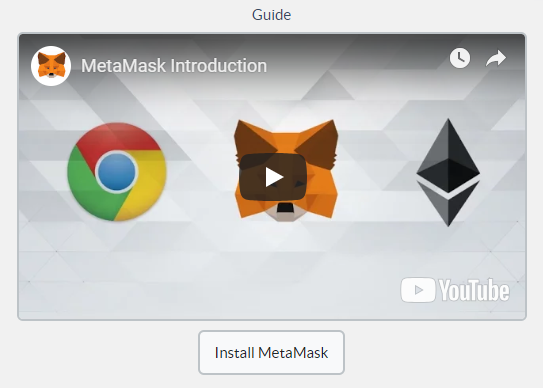
\includegraphics[width=7cm]{res/images/MetaMask_download.png}
		\centering
		\caption{MetaMask tutorial}
	\end{figure}
	\subsection{Configuration}
	To be able to use the site you also need a MetaMask account. Click on 
	MetaMask's icon on the top right of your browser, and set up your 
	personal wallet.\\
	You can either create a new one or import an existing one from the 12 
	words seed phrase.
	\begin{figure}[H]
		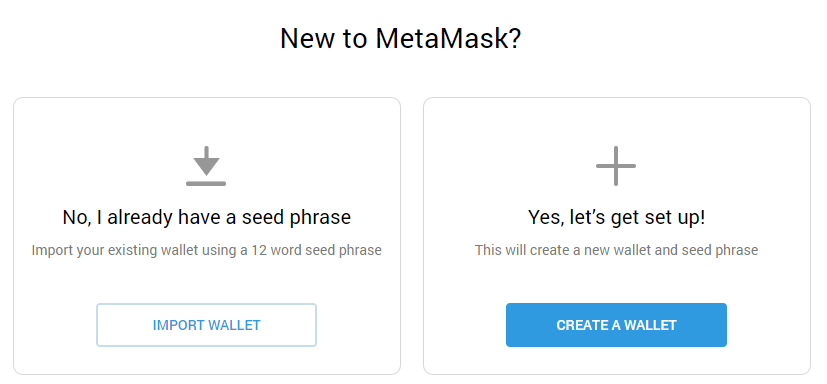
\includegraphics[width=7cm]{res/images/metamask_select.png}
		\centering
		\caption{MetaMask setup}
	\end{figure}
	\noindent After setting up your account you will be able to join and use 
	\textit{Soldino}.
	\newline \\
	Note that MetaMask has to be installed in your browser as long a you want 
	to use the platform, removing it from your browser will render you unable to
	use \textit{Soldino}.
	\subsection{Transactions}
	Every time you make a transaction MetaMask will show you its price and you 
	will be able to accept it or decline it.\\ \\
	%PLACEHOLDER ESEMPIO TRANSAZIONE
	Note that all prices shown are in Cubits, \textit{Soldino}'s own special token.
	Also remember that 1 Cubit = 1 Euro
%\section{First Use}
%	When you register in \textit{Soldino}, after entering your information, you 
%	have to allow the platform to access to your MetaMask information. When the 
%	pop-up window opens you must press "allow access" to use the site.
	%PLACEHOLDER inserire screenshot per permettere l'accesso
	
	
	
	